% !TEX root = ./report_entry.tex

\documentclass[./report_entry.tex]{subfiles}

\begin{document}
    
    \begin{titlepage}
        \noindent
        \centering \Huge \textbf{Satellite Track Fusion Using State Vector Classifer and Random Forest Voting Ensemble Model} \\
        CS 6840\\
        Ryan Arnold\\
        12/01/22
        \vspace{24pt}
        \clearpage
    \end{titlepage}  

    \section*{Introduction}

    \noindent In target tracking applications, sensor failure and sensor error can be a significant issue in
    data processing and object identification.  A method of mitigating this is to employ sensor fusion,
    which improves reliability by combining the data from multiple sensors.  This can
    overcome problems caused by noise and can offer higher accuracy and rubustness in classification.
    A key component of sensor fusion is the object classification step.
    A novel approach to the classification step is to employ machine learning.  For example, Vasuhi et al. demonstrated
    this capability by using State Vector Machine Classifiers (SVC) [1].
    \\ \\
    I attempted to extend the approach demonstrated by Vasuhi et al., by utilizing an SVC model approach in conjunction with
    an ensemble model.  Furthermore, I combined SVC models with Random Forest models (RF) on simulated satellite radar tracks
    using a voting classifier. For each sensor in my experiment, I fit a unique voting classifier ensemble model, and then combined the models together
    for a cumulitive prediction matrix. 
    Using a machine learning technique like this can offer higher performance on more complex datasets than conventional techniques [1].
    \clearpage

    \section*{Dataset}
    \noindent Using the Python3 library \textit{poliastro}, I simulated the orbital trajectories of three arbitrary satellites.
    This was performed using a Low-Earth-Orbital (LEO) model with a Keplian Orbit, using Earth as the main body.  I iteratively chose
    the paramters until I visually observed an intersection between the three orbital paths.  To stress the machine learning model,
    it was desirable to have a dataset with overlap to make it nontrivial to distinguish between tracks with their associated satellite objects.
    This was specifically configured by setting the initial velocity and position vectors for the three satellites in an inertial coordinate frame.
    After fitting the orbital models using the \textit{poliastro} api, the data was exported by extracting the resulting ephemeris data
    (time, position, velocity). The data was also exported to \textit{czml}, a json-like formatted file that can by read and rendered by Cesium Ion
    software.  A snippet of the python implementation is shown below:

    \begin{verbatim}
        from poliastro.twobody import Orbit

        orbit = Orbit.from_vectors(Earth, self.r, self.v, 
            epoch=START_TIME)
        ...
        ephem = orbit.to_ephem(strategy=EpochsArray(
            epochs=time_range(start=CROSS_START_TIME, end=CROSS_END_TIME, 
            periods=NUM_TIMES
        )))
        ...
        export_cesium(<filename>)
    \end{verbatim}

    The Cesium Ion Rendered depiction of the simulated dataset can be viewed in Figure \ref{cesium}.
    \clearpage

    \begin{figure}[!htbp]
        \centering
        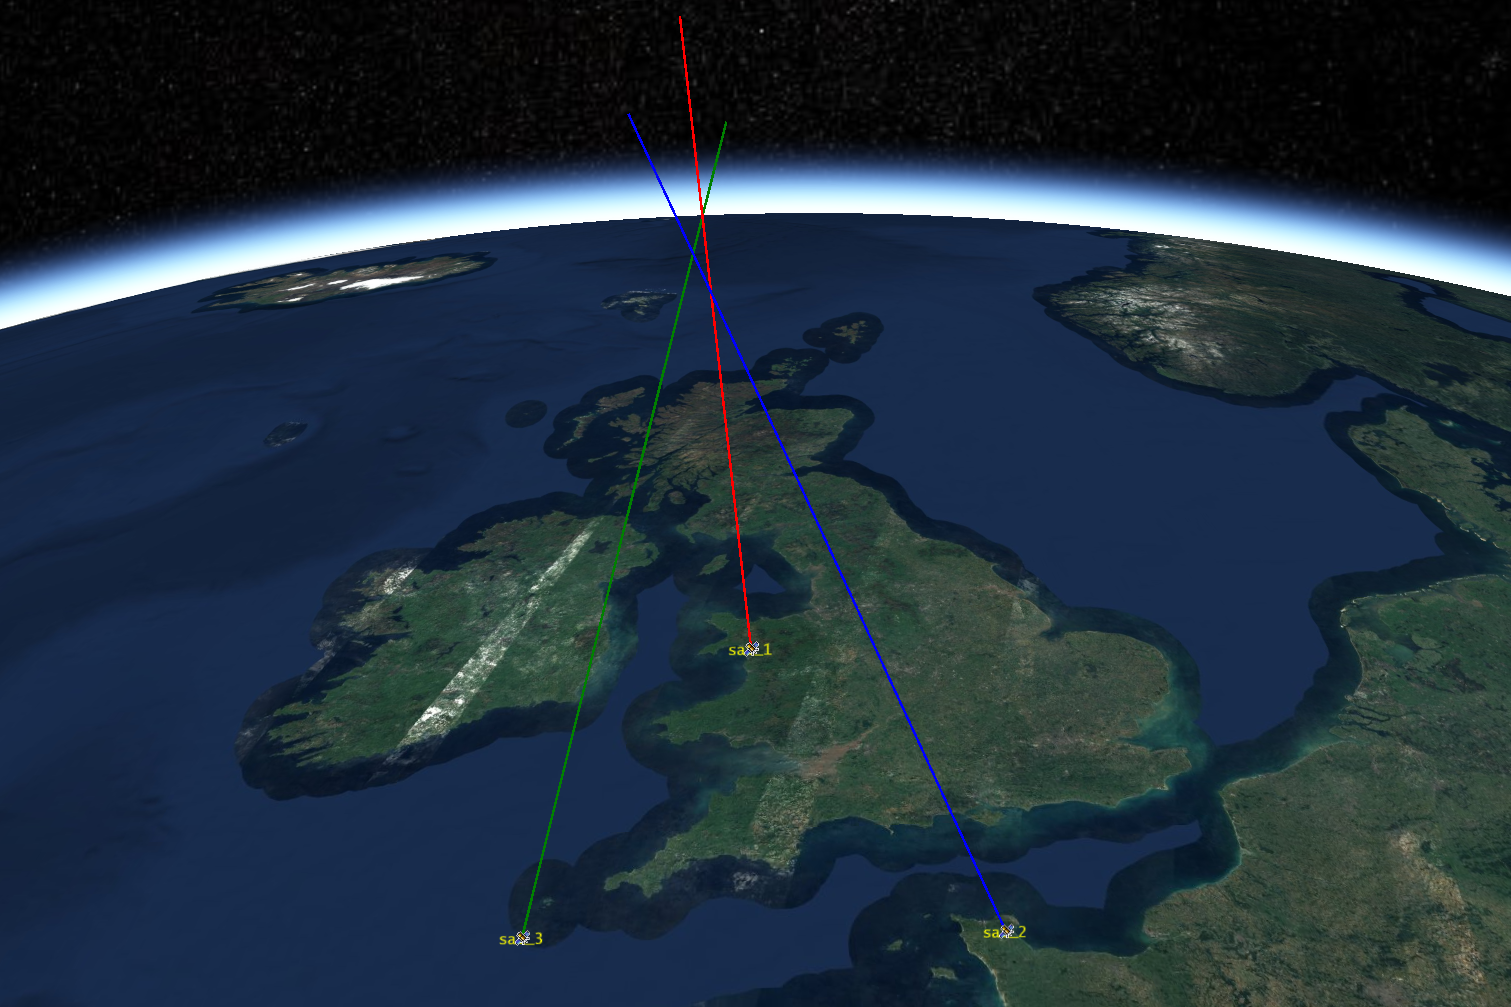
\includegraphics[scale=0.43]{../graphics/cesium2.png}
        \caption{Track Data Rendered in Cesium Ion Server.}
        \label{cesium}
    \end{figure}

    \noindent In this experiment, two fictitious radars were used.  This was accomplisehd by setting \textit{radar\_1} to 
    have a range error of $1km$ and \textit{radar\_2} to have a range error of $5km$.  Each radar contained 1500 observations, for a grand total of
    3000 observations.  When examining the dataset by satellite, there were 1000 observations per satellite object.  By using a random number generator,
    the original dataset was randomly split into two, equally sized, subsets to emulate two observation datasets from different radars.
    See the partitioning strategy in the example python code below:
    
    \begin{verbatim}
        ind = np.random.randint(len(RADAR_ERRORS._fields), 
            size=states[0].shape)
    
        for i, field in enumerate(RADAR_ERRORS._fields):
            # assuming the states are uniformly dimensioned
            
            epsilon: float = getattr(RADAR_ERRORS, field, 0.0)
            noise = np.zeros(states[0].shape) * units.km
            
            noise_ind = ind == i
            num_err = noise_ind.sum()
            noise[noise_ind] = epsilon * np.random.randn(num_err)
            
            for state in states:
                # attempt to normalize
                state.normalize()
                state.range_km += noise
    \end{verbatim}

    \noindent Before performing any machine learning algorithms, the data was pre-processed using the \textit{pandas}
    python api, after consolidating the ephemeris data to a \textit{pandas.DataFrame}. 
    The dataset was organized by time, spatial position(x,y,z), \textit{satellite\_id}, and \textit{radar\_id}.
    The input feature space consisted of 3-D cartesian positions $(x,y,z)$, with a 1-D label dimension using the \textit{satellite\_id} as the feature label.
    The data was partitioned into separate subsets based on \textit{radar\_id}.
    The results are dispayed in Figure \ref{hist} and Tables \ref{panda_head}-\ref{features}.
    \clearpage
    \begin{table}[]
        \centering
        \caption{Data Preview using DataFrame.head()}
        \begin{tabular}{l|llllll}
            \cline{2-6}
          & satellite\_id & radar\_id & time\_rel\_s & x\_km      & y\_km        & z\_km       \\ \hline
        0 & sat\_1        & radar\_1  & 10.000000    & 633.321711 & -5363.930987 & 5014.454006 \\
        1 & sat\_1        & radar\_1  & 10.005005    & 633.127425 & -5362.304441 & 5012.983412 \\
        2 & sat\_1        & radar\_1  & 10.010010    & 633.225240 & -5363.151863 & 5013.825616 \\
        3 & sat\_1        & radar\_1  & 10.015015    & 633.128131 & -5362.348358 & 5013.124427 \\
        4 & sat\_1        & radar\_2  & 10.020020    & 632.900068 & -5360.435713 & 5011.386305 \\ \hline
        \end{tabular}
        \label{panda_head}
    \end{table}
    \begin{table}[]
        \centering
        \caption{Data Summary Statistics}
        \begin{tabular}{l|llll}
            \cline{2-5}
              & time\_rel\_s & x\_km       & y\_km        & z\_km       \\ \hline
        count & 3000.000000  & 3000.000000 & 3000.000000  & 3000.000000 \\
        mean  & 12.500000    & 631.079652  & -5354.205352 & 5022.489484 \\
        std   & 1.445061     & 2.604249    & 8.065200     & 8.582994    \\
        min   & 10.000000    & 626.667610  & -5374.651893 & 5000.146205 \\
        25\%  & 11.250000    & 629.331781  & -5360.419547 & 5015.774211 \\
        50\%  & 12.500000    & 630.209829  & -5354.327071 & 5022.429047 \\
        75\%  & 13.750000    & 632.237250  & -5348.121667 & 5029.226351 \\
        max   & 15.000000    & 639.474429  & -5330.217558 & 5045.998444 \\ \hline
        \end{tabular}
        \label{stats}
    \end{table}
    \begin{table}[]
        \centering
        \caption{DataFrame Feature and Label Descriptions}
        \begin{tabular}{l|lll}
            \hline
        \# & Column        & Non-Null Count & Dtype   \\ \hline
        0  & satellite\_id & 3000 non-null  & object  \\
        1  & radar\_id     & 3000 non-null  & object  \\
        2  & time\_rel\_s  & 3000 non-null  & float64 \\
        3  & x\_km         & 3000 non-null  & float64 \\
        4  & y\_km         & 3000 non-null  & float64 \\
        5  & z\_km         & 3000 non-null  & float64 \\ \hline
        \end{tabular}
        \label{features}
    \end{table}
    \clearpage
    % put more text here probably
    \begin{figure}[!htbp]
        \centering
        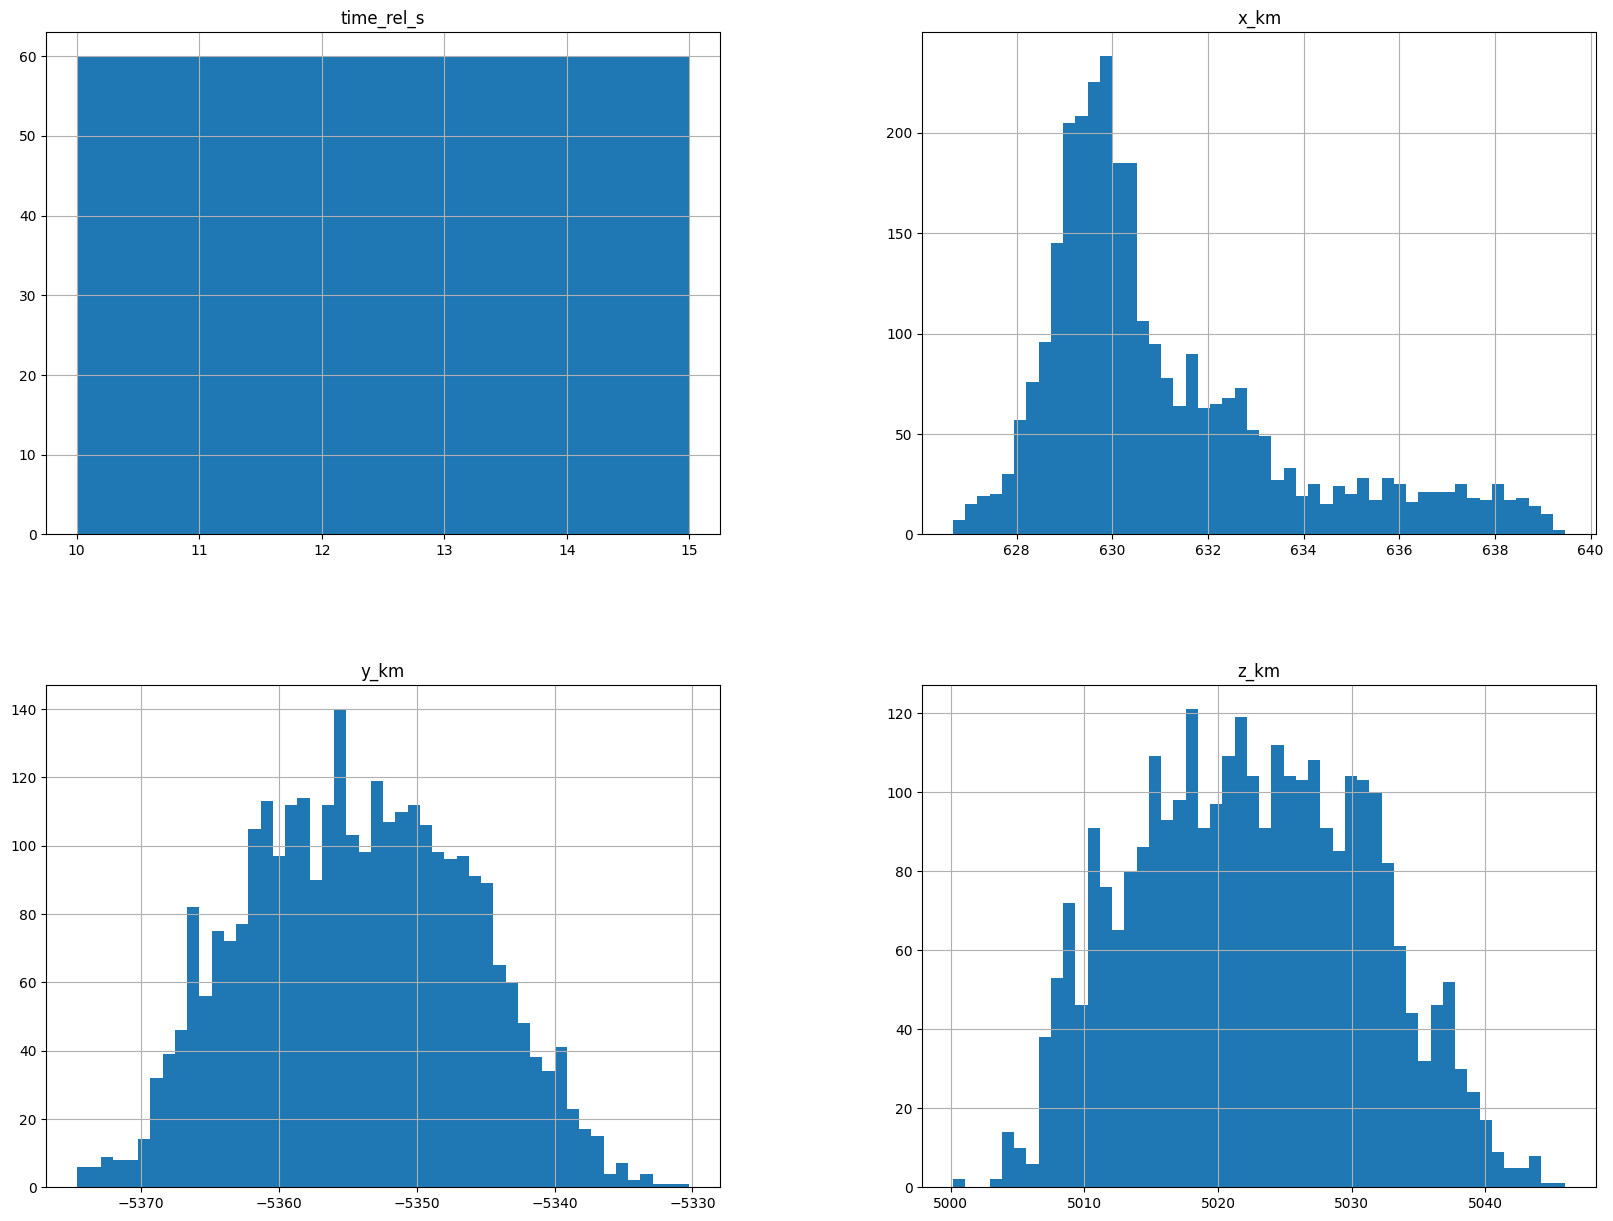
\includegraphics[scale=0.43]{../graphics/pre_proc.png}
        \caption{Histograms of input Features.}
        \label{hist}
    \end{figure}

    \noindent As presented in Figure \ref{hist}, the datasets are mostly evenly distributed.
    However, the x position dataset seems to be skewed left, with a concentration in the 
    lower component range in $[km]$.  Since the range errors were generated using Python Gaussian algorithms,
    it was expected that the data would mostly be evenly distributed.
    \\ \\
    \noindent The plot in Figure \ref{feature_plot} is the compilation of the two radar feature sets in one viewing space.
    The colors represent the different satellite objects, and the marker symbols represent the two
    radar groups.  Note the overlapping region of data near the center.  This is the critical region, where
    the machine learning model decision functions become more strained.

    \begin{figure}[!htbp]
        \centering
        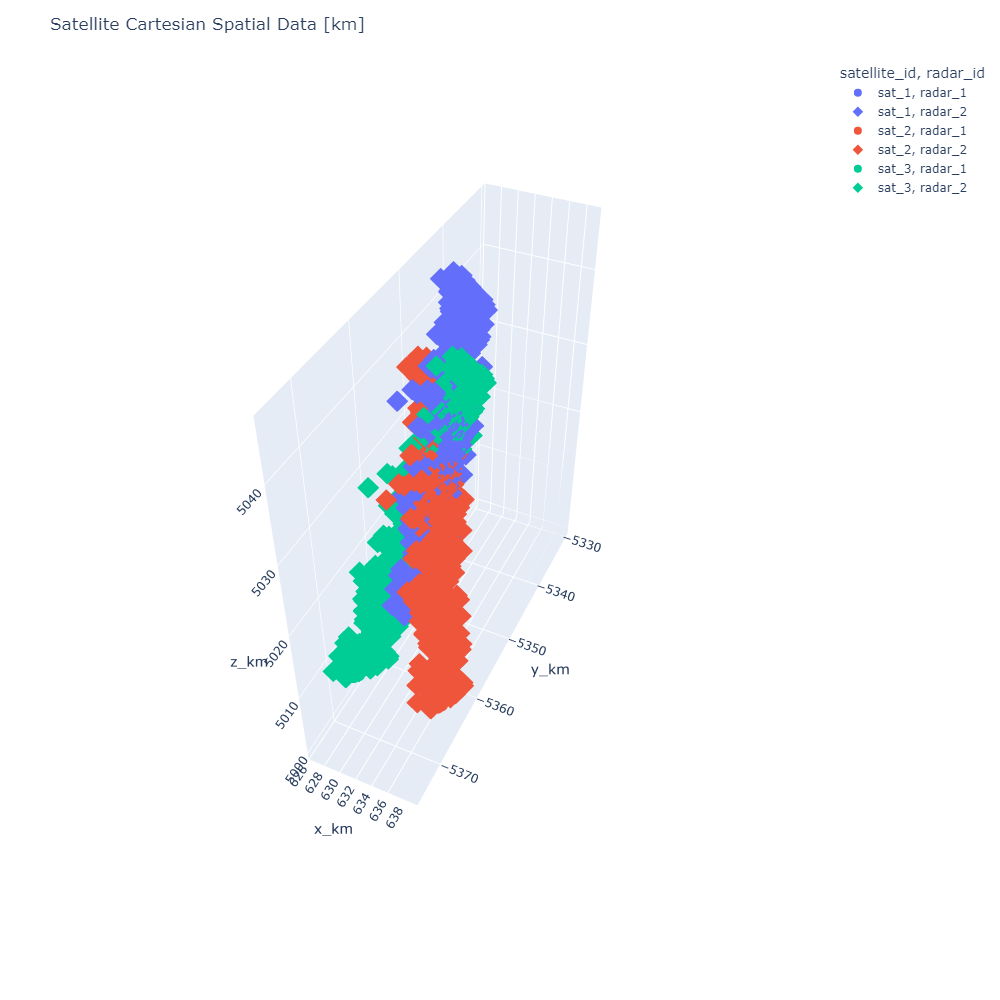
\includegraphics[scale=0.43]{../graphics/overlap.png}
        \caption{Combined Feature Space.}
        \label{feature_plot}
    \end{figure}

    \clearpage
    \section*{Methods}
        \subsection*{Primary Python Libararies}
            \begin{itemize}
                \setlength{\itemsep}{0pt}%
                \setlength{\parskip}{0pt}%
                \item astropy
                \item czml3
                \item matplotlib
                \item numpy
                \item pandas
                \item plotly
                \item poliastro
                \item scikit-learn
                \item tabulate
            \end{itemize}

        \subsection*{Methodology}
        \noindent The primary strategy for fusion involved finding an optimal shallow learning model for each radar, and
        subsequently fusing the predictions from each radar data subset.  The predictions from each radar were combined in a 
        cumulitive DataFrame, and used for the final classification results.  For each radar data subset,
        both a RF and SVC model were applied to the training datasets.  The training data and test data were split using a
        $80\%/20\%$ split respectively, via the \textit{sklearn.model\_selection.train\_test\_split()} method.
        \\ \\
        \noindent Each sub-model was hypertrained by passing hyperparameter ranges to the 
        \textit{sklearn.model\_selection.GridSearchCV} method.  This performed and exhaustive ''fit'' and ''score'' search
        to determine the optimal hyperparameters for each model with the provided training data.  After each model was fit for a given
        radar subset, the optimized models were passed togehter to a vote-based bagging ensemble method: \textit{sklearn.ensemble.VotingClassifier}.
        The voting classifier object selected the best model for the subset, based on a hard vote, using the mean
        accuracy as the metric criterion.
        \\ \\
        \noindent After the final voting classifiers were fitted for each radar subset, the predictions were combined
        between the two voting classifiers to get a comprehensive prediction DataFrame. The models were assessed by using 
        accuracy, macro F1 score, and total loss values.  For the Rf models, a log-loss function was used; for the SVC models, a
        hinge-loss function was used. As a pre-emptive observation, the two models performed similarly.  Also, considering the skewness of the X
        feature dimension, it was deemed necessary to run several fits and average the final results to properly assess model performance.  Training and testing
        data splits were constructed using stratified k-fold splits via the \textit{sklearn.model\_selection.StratifiedShuffleSplit}
        method.  A total of 10 splits were fitted, and the model fitting scores were averaged.  In addition, the winnning models for
        each split were tabulated.  Confusion matrices were also computed to better visualize the model performances.
        \\ \\
        \noindent A sample snapshot of the model code is shown below:

        \begin{verbatim}
            grid_search = GridSearchCV(
                svm.SVC(),
                params_grid,
                cv=5,
                n_jobs=-1,  # run jobs in parallel to speed things up
                #scoring='neg_mean_squared_error',
                return_train_score=True,
                verbose=3
            )

            ...

            # retain only the spatial data
            X = subset.drop(
                columns=['satellite_id', 'radar_id', 'time_rel_s'])
            y = subset.satellite_id
            
            X_train, X_test, y_train, y_test = train_test_split(
                X, y, test_size=0.2, random_state=RANDOM_STATE
            )
            
            if not final_cache_filename.is_file():
                clf_svc = fit_svc(X_train, y_train,     
                    svc_cache_filename)
                clf_rf = fit_random_forest(X_train, y_train, 
                    rf_cache_filename)
                
                estimators = [('svc', clf_svc), ('rf', clf_rf)]
                clf = VotingClassifier(estimators, voting='hard')
                clf.fit(X_train, y_train)
        \end{verbatim}

    \section*{Experimental Results}

            \begin{table}[htbp]
                \centering
                \caption{K-Fold Experiment Results: Radar 1 (K=10)}
                \begin{tabular}{|c|c|}
                    \hline
                    \multicolumn{2}{|c|}{\textbf{Radar 1}} \\ \hline
                    Total Times SVC Chosen & Total Times RF Chosen \\ \hline
                    7 & 3 \\ \hline
                \end{tabular}
                \label{k-radar1}
            \end{table}

            \begin{table}[htbp]
                \centering
                \caption{K-Fold Experiment Results: Radar 2 (K=10)}
                \begin{tabular}{|c|c|}
                    \hline
                    \multicolumn{2}{|c|}{\textbf{Radar 2}} \\ \hline
                    Total Times SVC Chosen & Total Times RF Chosen \\ \hline
                    2 & 8 \\ \hline
                \end{tabular}
                \label{k-radar2}
            \end{table}

            \begin{table}[htbp]
            \centering
            \caption{Final Model Results: \textbf{Radar 1}}
            \begin{tabular}{cccc}
                \hline
                Classifier & Accuracy & Loss [hinge-SVC/log-RF] & Macro F1 Score \\ \hline
                SVC & 0.970684 & 1.75211 & 0.96994 \\
                RF & 0.970684 & 0.123589 & 0.969483 \\ \hline
                \end{tabular}
                \label{final_radar_1}
            \end{table}

            \begin{table}[htbp]
                \centering
                \caption{Final Model Results: \textbf{Radar 2}}
                \begin{tabular}{cccc}
                    \hline
                    Classifier & Accuracy & Loss [hinge-SVC/log-RF] & Macro F1 Score \\ \hline
                    SVC & 0.935374 & 2.22855 & 0.926926 \\
                    RF & 0.911565 & 0.235218 & 0.909554 \\ \hline
                    \end{tabular}
                    \label{final_radar_2}
            \end{table}

            \begin{figure}[!htbp]
                \centering
                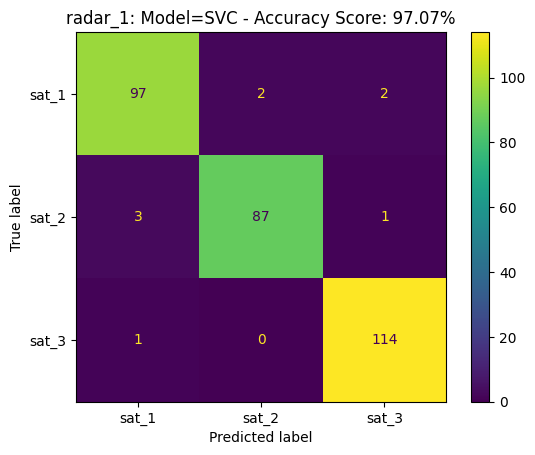
\includegraphics[scale=0.80]{../graphics/CM_radar1.png}
                \caption{Confusion Matrix Ensemble Classifier Radar 1.}
                \label{cm1}
            \end{figure}

            \begin{figure}[!htbp]
                \centering
                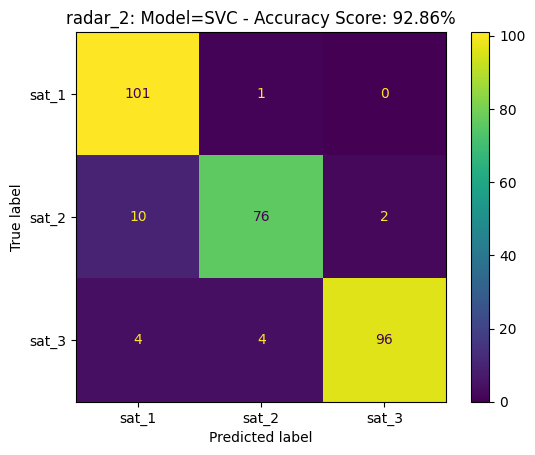
\includegraphics[scale=0.80]{../graphics/CM_radar2.png}
                \caption{Confusion Matrix Ensemble Classifier Radar 2.}
                \label{cm2}
            \end{figure}

            \begin{figure}[!htbp]
                \centering
                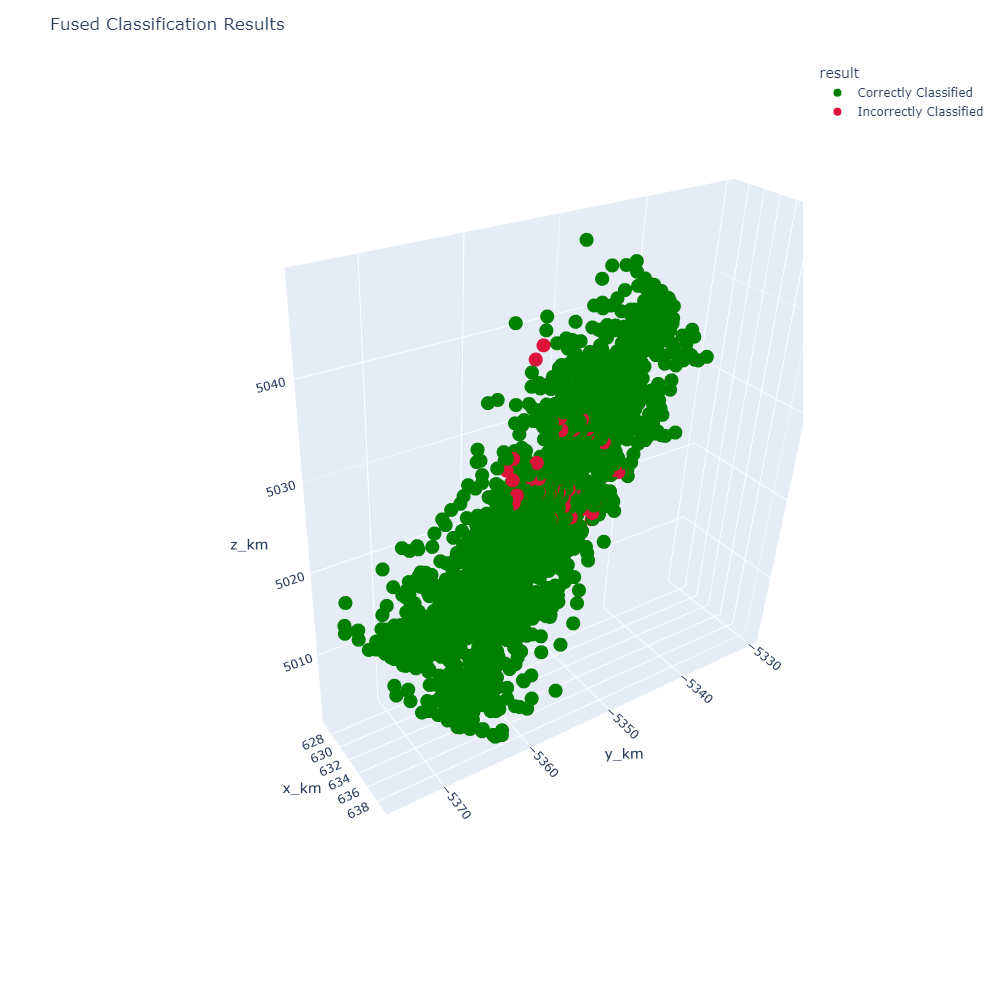
\includegraphics[scale=0.45]{../graphics/final_class.png}
                \caption{Confusion Matrix Ensemble Classifier Radar 2.}
                \label{final}
            \end{figure}
    \section*{Discussion}

        \noindent All of the final enesmble models had accuracies $>90\%$, which are promising resutls.  In the 
        experiemnt using a single randomized train/test split method, the SVC model slightly outperformed the RF model.  
        However, this was insignificantly better in the Radar 1 subset and approximately $2.4\%$ in the Radar 2 subset (see Tables \ref{final_radar_1} and \ref{final_radar_2}).
        Given the similarity in performance, it is more insightful to inspect the results of the k-fold analysis, where
        the models were fit to training data multiple times with different folds.
        \\ \\
        \noindent Interestingly, the RF model actually outperforms the SVC model a majoriy of the time with the Radar 2 subset ($80\%$), and 
        $30\%$ of the time for Radar 1 (See Tables \ref{k-radar1} and \ref{k-radar2}).  The distinguising parameter of Radar 2 was the higher range error (five times that of Radar 1).  It
        is possible that The RF model performs better on noiser datasets than the SVC model.  This is likely due to 
        the state vectors being more error prone in noiser environments.  When there is not a clear distinciton between 
        the feature sets, it is more difficult to establish a hyperplane that can properly spatially separate the features.
        Conversely, the RF model does not have such strict spatial dependence as the SVC model, so it makes sense that the noiser spatial data would
        be easier to separate using an RF model.
        \\ \\
        \noindent Both confusion matrices in Figures \ref{cm1} and \ref{cm2} had satisfactory results, with a high
        concentration of True Positive predictions.  The only noteworthy error was for Radar 2 in Figure \ref{cm2}, there seemed to be a
        disproportionatly high amount of False Positives for satelltite 1, when the true object was satellite 2.  Overall, according to the fused results
        displayed in Figure \ref{final}, the model seemed to have the most trouble accurately classifying the objects 
        in the overlapping region, concentrated mostly at the center.  This is indicated by the presence of red markers in this regime.
        This was expected, given the close proximity of the points in that region, making it difficult to calculate rigid decision boundaries.
        The presence of noise/error further complicates the decision boundary formation.

    \section*{Challenges and Future Steps}
        \noindent The biggest challenge of this project computationally was the hypertraining via the Sklearn grid search
        implementation.  When I used finer parameter ranges within the grid, the program would often get stuck on threads,m
        making it impossible to optimize the parameters for that resolution.  Optimizing the code, using better hardware, or allowing more 
        computation time may have improved this.
        \\ \\
        \noindent  Another challenge was defining the ratio of overlapping points to non-overlapping points.
        Since the solution to the initial orbit parameters was done primarily throught trial and error, a more empirical solution
        would have been ideal.  Moreover, having a proper solution could allow for an examination of the proportion of overlapping points versus
        non-overlapping points, and how this would affect the model fitting/selection process.
        \\ \\
        \noindent In terms of future work, better preprocessing could have been performed.  For example, using techniques like PCA and data scaling, could have been
        implemented to better screen the data.  Other models could have been tested as well, instead of exclusively RF and SVC classification
        models.  A semi-supervised clustering algorithm could have also been insightful, since distance is an important parameter to that algorithm,
        and is makes intuitive sense to use as an optimization paramter for a spatial dataset.  Finally, in order to create a higher fidelity model, more advanced trajectories with a 
        higher object count and additional sensors should be tested.
    \section*{Conclusion}

            \noindent Using the \textit{poliastro} Python library, it was possible to simulate overlapping satellite trajectories for three satellites.
            To incorporate a track fusion algorithm, different radars were emulated by randomly splitting the track observations into equally sized subsets, and corrupting
            the data with range error noise, unique to two different radars.
            Overall, the ensemble model demonstrated high performance, with a mean accuracy of $97.0\%$ and $92.9\%$ for
            Radar 1 and Radar 2 respectively.  Given that the Radar 2 subset had a higher simulated measurement error,
            it was expected that performance would be lower.  Interestingly, according to the K-fold evaulation experiment,
            the Random Forest model outperformed the State Vector Machine Classification model for the noiser dataset associated with
            Radar 2.  Given that the RF model has less computational overhead, this model may be more desirable in applications
            that require high performance (such as real-time applications).  Also, if the dataset is more prone to measurement error,
            the RF model could be a better option, based on the results in Table \ref{k-radar2}.
    
    \clearpage
    \begin{thebibliography}{9}

        \bibitem{paper}
        Vasuhi, S., Vaidehi, V., Midhunkrishna, P. R. (2011). 'Multiple target tracking using Support Vector Machine and data fusion.' \textit{3rd International Conference on Advanced Computing, ICoAC} 2011, 407–411. https://doi.org/10.1109/ICoAC.2011.6165210
        
        \bibitem{towards_data_science}
        Paialunga Piero. "Ensemble Learning with Support Vector Machines and Decision Trees" \textit{Towards Data Science} (13 December 2020).
        https://towardsdatascience.com/ensemble-learning-with-support-vector-machines-and-decision-trees-88f8a1b5f84b   
    
    \end{thebibliography}

\end{document}